
\documentclass{article}
\usepackage{graphicx} % Required for inserting images
\usepackage{graphics}
\usepackage{subfigure}
\usepackage{hyperref}

\usepackage[firstpageonly]{draftwatermark}
\SetWatermarkText{DRAFT}
\SetWatermarkScale{8.5} % Adjust size
\SetWatermarkColor[gray]{0.85} % Light gray

\usepackage[linesnumbered,boxed]{algorithm2e}

\title{Temporal Computing}
\author{Jonny Edwards}

\date{\today}
\begin{document}
\maketitle
\begin{abstract}
	This report consists of a review of the literature and a plan for integration related to \textbf{temporal computing}, a novel method of computation that uses time intervals as the primary method of storing and manipulating data. The literature review covers a broad range of methods, with the plan of further work focusing on assessing a novel temporally inspired digital implementation of a probabilistic temporal architecture, which can be readily used at the layer below the MeTTa language.
\end{abstract}

\section{Introduction}
The ability to perform accurate repetitive computation has been central to numerous scientific and technological advances in the last seventy years. At the heart of this is Moore's Law \cite{Moore:2000:CMC:333067.333074}, which states that computational power provided by the silicon based Central Processing Units (CPUs) will double year-on-year for the foreseeable future. Unfortunately, several factors have compounded to make this less likely to continue: heat dissipation, atomic and quantum effects provide practical limits to the miniaturisation and packing of transistors \cite{moorefail}, and the limited bandwidth between CPU and memory limits computation speed (the von-Neumann bottleneck \cite{Backus:1978:PLV:359576.359579}). There is also doubt about  fabrication processes working below 3nm, although many vendors are issuing in even more miniaturisation which they refer to as the angstrom era (see Figure \ref{fig:intel}).


\begin{figure}[ht]
	\centering
	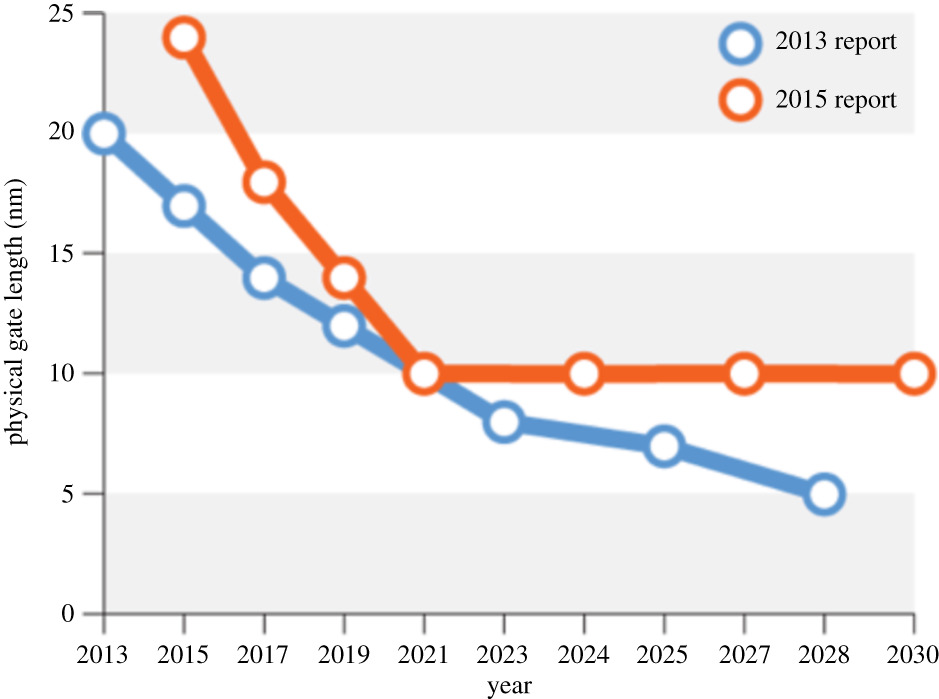
\includegraphics[width=200pt]{figures/intel2.jpg}
	\caption{Predicted physical gate size decline over the next five years. Credit: \url{https://doi.org/10.1098/rsta.2019.0061/}}
	\label{fig:intel}
\end{figure}

At the same time, methods of data processing using learning systems have become significant new architectural components. Of these, Deep Learning (DL) \cite{lecun2015deep} has provided best-in-class performance on many machine learning tasks, and revitalised many areas of pattern recognition, opening up a revolution in new services that were traditionally performed using human intensive processes. Moreover, these methods are not well supported by traditional computer architectures \cite{JEON2021167} as they require massive parallelism, similarly to the brain. Graphics Processing Units (GPUs) , initially built for video games, have been successfully utilised, but still suffer from high levels of inefficiencies which are many orders of magnitude away from biological systems in energy and ability.

Given this impasse, there is a need to look more broadly at the problem of improving the efficiency \textbf{and} accelerating computation. This has resulted in a ``Cambrian explosion'' \cite{hennessy2019new} of new approaches, and this research focuses on one of these, \textbf{ temporal computing}.

This new approach represents numbers with a unary encoding (discussed in more detail in Section \ref{unary}) instead of binary, and uses \textit{time delays} to represent data instead of digital bit manipulation. We are drawn to this area for several reasons.

\begin{enumerate}
	\item There is a precedence in nature, the human brain uses spike-based information as the main processing encoding \cite{victor2000brain}.
	\item Unary is more simplistic than binary to compute with. Tools such as the abacus are among the earliest calculators \cite{POPPELBAUM198747}.
	\item On the surface, time appears to be a free resource. For a typically coded temporal interval, the is only ever a requirement for two delimiting spikes (See Figure \ref{fig:two} ) \cite{smith2022temporal}.
\end{enumerate}

\begin{figure}[ht]
	\centering
	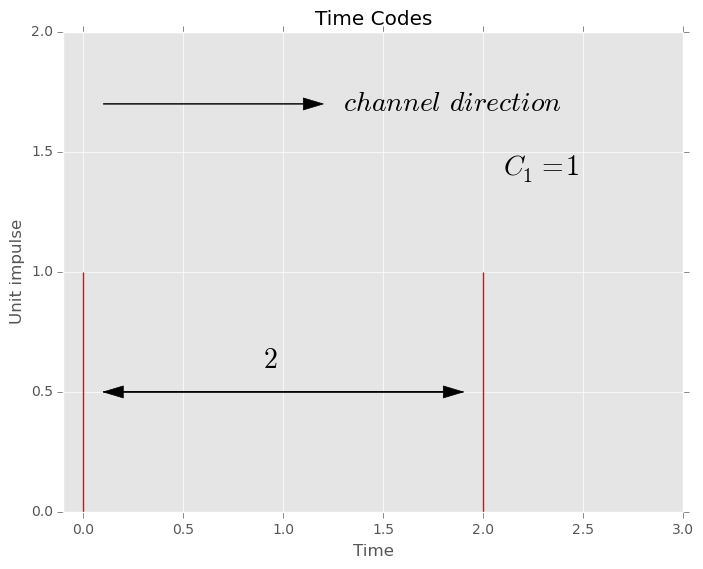
\includegraphics[width=200pt]{figures/logfig1.png}
	\caption{A typical value can be represented as two delimiting spikes.}
	\label{fig:two}
\end{figure}



The three capabilities detailed above provide a broad definition of an area of research, but this is yet to be established in the mainstream. Four areas: racelogic, unary processing, oscillatory Computing and neuromorphic compute, utilise time as a medium but do so without explicitly exploiting the above features. This is particularly the case with two areas under review, neuromorphic and oscillatory computing, with methods in these areas often conflating the benefits of hardware and problem specific algorithmic approaches.

The problem of defining temporal computing is further compounded by misuse of the term ``stochastic'' eg in works \cite{wu2020ugemm,wu2023power}, and significant oversight in not including previous work from the late sixties on unary compute \cite{POPPELBAUM198747}, in discussions.

With this in mind, the agenda of this report is:
\begin{itemize}
	\item To cover all research specifically referenced as ``temporal'' by the racelogic community (section \ref{race}). For completeness, include Unary, oscillatory and neuromorphic computing in the discussion (Sections \ref{oscil} and \ref{neuro})
	\item To pave the way for the integration of this work into a broader probabilistic framework that is amenable for integration into a declarative AGI pipeline such as that provided by the MeTTa language.
  	
\end{itemize}


\section{Racelogic} \label{race}
Racelogic is undoubtedly the most significant area of research in the temporal domain, both computation and memory, and has formed a small community in the US \cite{madhavan2014race}.

The central theme of this work is the utilisation of the two timing properties of traditional logic gates. Under a temporal scheme an \texttt{AND} gate acts as a \texttt{MAX} operation, and the \texttt{OR} gate acts as a \texttt{MIN} operation (see Figure \ref{fig:race}).


\begin{figure}[ht]
	\centering
	\subfigure[]{
		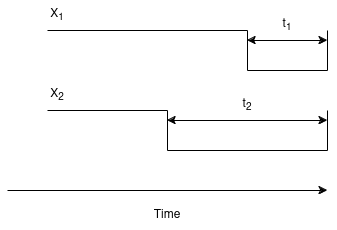
\includegraphics[width=200pt]{figures/racesignal.png}
	}
	\\
	\subfigure[]{
		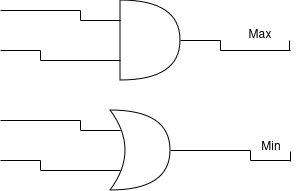
\includegraphics[width=200pt]{figures/minmax.png}
	}
	\caption{A visual explanation of racelogic. The first diagram shows the representation and second gives the ``race'' min/max effect}
	\label{fig:race}
\end{figure}


Using this a variety of systems have been proposed and implemented \cite{madhavan2014race}, most notably to perform minimum and maximum path search on a graph \cite{madhavan2015race}.

This work has been extended to utilise a tropical algebra \cite{madhavan2021temporal} a semi-ring that implements multiplication and addition, and this was referred to as a Temporal State Machine. Under this scheme various additional graph algorithms including Dikstra's were implemented and benchmarked.

Further work by this group also involved building temporal memories called \textit{Racetracks} \cite{vakili2020temporal,madhavan2020storing}. The basis of this is akin to dragging a bucket for a set distance, the time to do this becomes fixed for a set bucket size (see Figure \ref{fig:racetrack}). In this work this is implemented on a magnetic platform, with the addition of a recovery track to reset the memory. This is the first known implementation of memory and the ``dragging time'' approach seems to be something that could be readily applied in many resistive physical mediums.

\begin{figure}[ht]
	\centering
	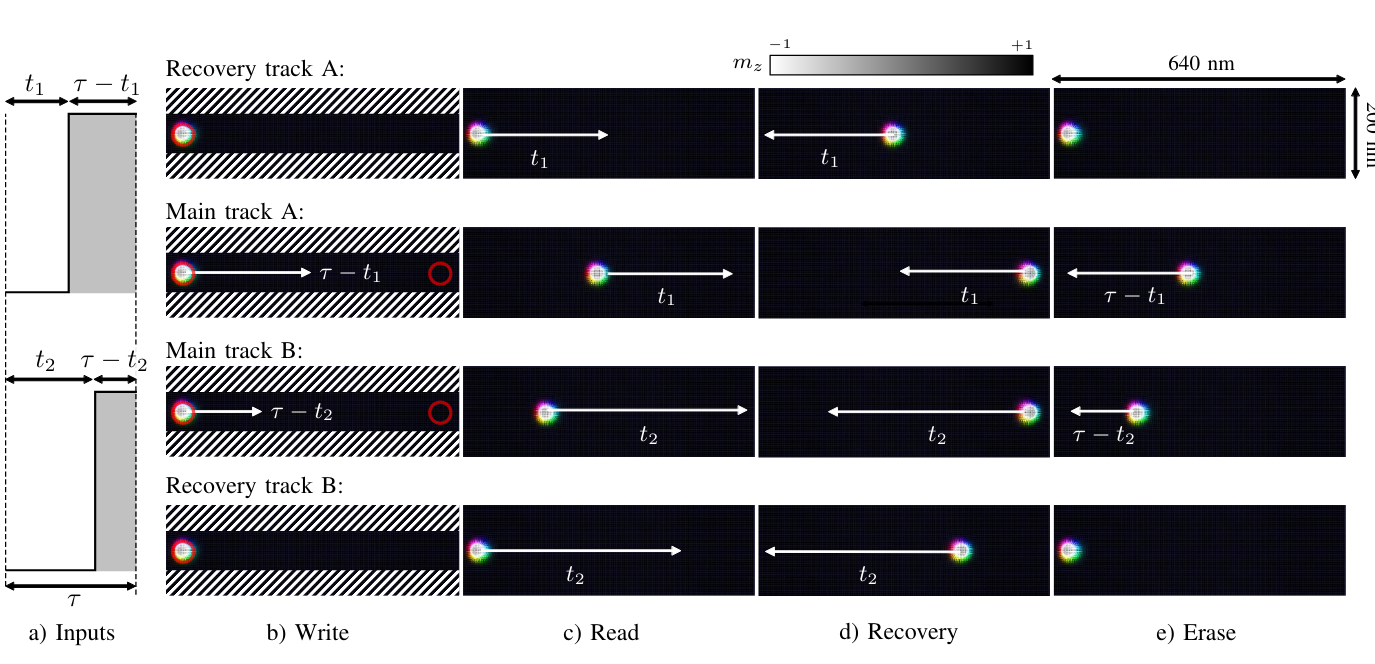
\includegraphics[width=300pt]{figures/racetrack.png}
	\caption{The racetrack memory operations. Taken from \cite{vakili2020temporal}}
	\label{fig:racetrack}
\end{figure}

The logic gate processing format has also been explored by two further parties, in the context of superconducting mediums \cite{tzimpragos2019arbitrary} \cite{tzimpragos2021temporal} \cite{tzimpragos2022computing} \cite{volk2023addressable} \cite{segal2022digital} also as a formulation for a specific supporting algebra. The superconducting work follows a similar pattern and is limited to a constrained view of logic operations applied to temporally organised inputs. This work is excellent proof-of-concept work, but lacks reference to comparable digital algorithms and the nature of space/time trade-offs.

\section{Unary Computation} \label{unary}

Unary number systems (\cite{MacKay:2002:ITI:971143} Chapter 7 page 133) were amongst the earliest numerical representations of quantity, with the abacus existing as the earliest calculating device \cite{POPPELBAUM198747}. Unary codes are a simplification, with either binary digit acting as the delimiter. Table \ref{mem1} gives a breakdown of how unary codes are constructed for the first few decimal numbers. We introduce a further code Discrete Pulse Interval Modulation (DPIM), which is a form of unary code, and is used in the communication community.

\begin{table}[ht]
	\begin{center}
		\begin{tabular}{rlll} \hline
			\textbf{Decimal} & Unary (U) & Unary code (UC) & DPIM             \\\hline
			\textbf{0}       &           & (0) may delimit & (11) may delimit \\
			\textbf{1}       & 1         & 1               & 101              \\
			\textbf{2}       & 11        & 10              & 1001             \\
			\textbf{3}       & 111       & 100             & 10001            \\ \hline
		\end{tabular}
	\end{center}
	\caption{Coding Schemes related to Temporal Computing}\label{mem1}
\end{table}


One of the key benefits for all the unary family is that simple arithmetic is easily derived: Addition with unary, as with the abacus, is performed trivially using simple concatenation \cite{jonny1}.

Integer multiplication of unary codes is performed by dilating the first unary code by the size of the second code. In a fully clock based architecture this can be performed by changing the relative clock speeds of the sender and receiver of the signal (see \cite{jonny1} section 3.3 for a more detailed explanation)  Again, this is a simple operation which requires only basic logic to perform.

The review paper of Poppelbaum \cite{POPPELBAUM198747} explains in some detail first-generation unary computers. There are three types of unary processing: stochastic, burst and pulse gear based approaches. These systems can be summarised as follows:

\begin{description}
	\item[Stochastic] where the unary value represents a discrete probabilistic range, sometimes with randomness incorporated. Many machines have been built with this premise, including \textbf{RASCEL} \cite{esch1969rascel} \textbf{POSTCOMP} \cite{poppelbaum1967stochastic}. This continues to be an active field of research \cite{alaghi2013survey}. We review this work in more detail below.

	\item[Burst] This is more akin to traditional unary but with a specific bit-width, so for instance 7 out of 10 bits set (\texttt{1111111000}) would equal 7. Examples of it's use are \textbf{BURST} \cite{POPPELBAUM198747} and \textbf{WALSHSTORE} \cite{bracha1978walshstore}.
	\item[Pulse Gear] This again uses burst unary but provides a clever method for shifting and ANDing to perform operations. An example of this is the \textbf{UNIFIELD} processor \cite{dollas1987architecture}.
\end{description}


These largely forgotten systems are all very interesting applications of unary and could be utilised in the design of new processing elements, the Pulse Gear methods, and the use of AND gates and counters have some resonance with methods discussed later in this review.

Two further points should be noted. Firstly, none of these systems use the benefits of redundancy and the delimiting nature of unary codes and are firmly wedded to using many boolean \texttt{on} (\texttt{1}'s) values. Secondly they are explicitly non-temporal, this means that time is not used to represent data.

More modern work in this area has been performed by Wu \cite{wu2020ugemm} \cite{pan2022t} \cite{wu2022usystolic}. This work is again mainly unary and again not explicitly temporal.

Before moving on to more elaborate unary notations, let us briefly discuss stochastic and probabilistic methods. In stochastic computing,a form of unary encoding is performed using random bitstreams where the proportion of 1s represents a numerical value. This is typically done using either \textbf{unipolar} or \textbf{bipolar} encoding schemes.
Unipolar Encoding represents values in the range $[0, 1]$. A number $x$ is encoded as a bitstream where the probability of a 1 is $x$. For example, a value of $0.75$ might be encoded as a bitstream like \texttt{1101111011111011}, which contains approximately $75\%$ 1s. A Bipolar Encoding Represents values in the range $[-1, +1]$. A value $x$ is encoded with the probability of a 1 as $(x + 1)/2$. For example, a value of $-0.5$ would be encoded with a bitstream containing approximately $25\%$ 1s.

\subsubsection{Advantages}
\begin{itemize}
  \item \textbf{Simplified arithmetic:} Multiplication becomes a simple AND gate (unipolar) or XNOR gate (bipolar).
  \item \textbf{Fault tolerance:} Randomness makes systems robust to noise and bit flips.
  \item \textbf{Low hardware cost:} Uses simple logic gates instead of full arithmetic units.
\end{itemize}

\section{Example: Unipolar Multiplication}
To multiply $0.5 \times 0.75$:
\begin{itemize}
  \item Encode $0.5$ as a bitstream with $50\%$ 1s.
  \item Encode $0.75$ as a bitstream with $75\%$ 1s.
  \item AND the streams to get a result with approximately $37.5\%$ 1s, representing $0.375$.
\end{itemize}

\section{Challenges}
\begin{itemize}
  \item \textbf{Accuracy:} Requires long bitstreams for precision.
  \item \textbf{Latency:} Longer streams mean slower computation.
  \item \textbf{Correlation:} Input streams must be uncorrelated to avoid bias.
\end{itemize}

A \textbf{p-bit} (probabilistic bit) is a classical binary unit that fluctuates randomly between $+1$ and $-1$ with a tunable probability. Unlike deterministic bits, p-bits are inherently stochastic and can be biased toward one state or the other using an input signal \cite{camsari2017stochastic}.

\subsubsection{Mathematical Model}
The state $m_i$ of a p-bit is given by:

\begin{equation}
	m_i(t) = +/- [\tanh(I_i(t)) + r(t)]
\end{equation}
where:
\begin{itemize}
  \item $I_i(t)$ is the input bias at time $t$
  \item $r(t)$ is a random number uniformly distributed in $[-1, 1]$
  \item $+/-$ is the sign function
\end{itemize}

\subsubsection{Key Properties}
\begin{itemize}
  \item \textbf{Tunable randomness:} The probability of outputting $+1$ or $-1$ depends on the input bias.
  \item \textbf{Autonomous flipping:} P-bits update asynchronously and independently \cite{camsari2019petaflips}.
  \item \textbf{Energy-efficient:} Can be implemented using low-power devices like stochastic magnetic tunnel junctions (sMTJs) \cite{camsari2023fullstack}.
\end{itemize}

\subsubsection{Comparison to Stochastic Computing}
While both p-bits and stochastic computing rely on randomness, p-bits  Operate on single fluctuating bits rather than long bitstreams, and allow dynamic tuning of probability via input bias. They are better suited for asynchronous, parallel architectures.

It is easy to envision p-bits in a temporal unary setting, utilising a time axis for the storage of the probabilistic value. We will refer to these as \textbf{pt-systems}. This is thus-far uncharted territory, with no existing system using this as a methodology, and this is the key area we aim to explore in the design of a new temporal system.

\subsection{Multiplexed Unary}

\textbf{Unary codes} have an additional property that a set of non-duplicate values can be efficiently multiplexed. Again to use the abacus analogy, if we have beads of two colours: black ($1$) and white ($0$), provided there is no duplication, multiplexing can occur which \textit{reuses white beads}. Again, the logic of this is a simple \texttt{OR}ing of the value from a start reference bit. Figure \ref{fig:mul1} presents this graphically. This system is \emph{genuinely} multiplexing; the two values are overlaid so the values actually forms part of the subsequent data. This is unique to this coding strategy and is unlike any other system of multiplexing. The general algorithm for conversion to this multiplexed domain is as follows:


\begin{figure}
	\centerline{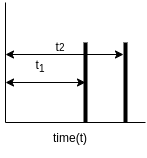
\includegraphics[width=100pt]{figures/multiplex.png}}
	\caption{An example of genuine multiplexing}\label{fig:mul1}
\end{figure}

\begin{algorithm}
	%\SetLine % For v3.9
	\SetAlgoLined % For previous releases [?]
	\For{each value I in C}{
		At position I in MUX window append $1$\;
	}
	\caption{Encoding Algorithm}
\end{algorithm}

Once transformed, signals can be interleaved in such a way that they can be easily recovered. To de-multiplex, the process is reversed, with the MUX channel progressively reconstructs the input values back into separate channels.

\begin{algorithm}
	%\SetLine % For v3.9
	\SetAlgoLined % For previous releases [?]
	\For{0..$I$} {
		\If 1 {
				Write I into output channel;
			}
	}
	\caption{Decoding Algorithm for DMU}
\end{algorithm}


A natural extension is to enable the unary coded $1$ value to be multi-valent. Although at first this may appear contrived, the motivation for this is the extension of the multiplexing method to incorporate duplicates, and the ability to better encode analog interval channels. This channel also has an additional property that multiplication can be performed, at least within the bounds of the notation, by placing a value $a$ at position $t$, and \textit{also} multiplexing as in Figure \ref{fig:multiply}.


\begin{figure}[ht]
	\centerline{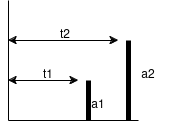
\includegraphics[width=100pt]{figures/multiplex2.png}}
	\caption{Multi-valent multiplexing for a potential analog implementation}\label{fig:multiply}
\end{figure}

Although not immediately obvious, an uncertainty relationship exists between position and data when ``dense'' multiplexing is used. To illustrate this let us take the trivial sequence (1,3,2) with knowledge of the prior this could be easily transformed into the densely multiplexed representation of (111) \footnote{1=1,2=01,3=001} which notionally can be represented with a smaller number of bits, but with a loss of order in the data. Adding positional values via a positional index recovers from the problem but at the cost of extra data, with a different prior distribution.

Clearly, the act of multiplication can be transformed into manipulating the values held in the buckets. This can be easily extended to a dot-product operation and the representation of tuple pairs is somewhat compressive since one element of the 2-tuple is specified by a positional index.

Under a simple scheme, tuples can be added arbitrarily to the array at their $t$ index point.  A dot product on this multiplexed array can be evaluated efficiently and in a systolic way using the \textbf{Multiplicative ADD} (MADD) algorithm (Algorithm \ref{madd}) as shown in \cite{jonny-asynch}. Figure \ref{fig:madd} demonstrates that the algorithm is effectively finding the area of the rectangles $4 \times 10$ and $4 \times 4$ by progressively sweeping in one pass back across the indexed array, counting initially the first $6 \times 4$ and then the remaining $8 \times 4$.

\begin{algorithm}
	$acc,height \gets 0$\;
	$i \gets |mem|-1$\;
	\While{$i>0$}{
		$height \gets height + mem[i]$\;
		$acc \gets acc + height$\;
		$i \gets i-1$\;
	}
	\textbf{return} acc
	\caption{The MADD algorithm} \label{madd}
\end{algorithm}

\begin{figure}[ht]
	\centerline{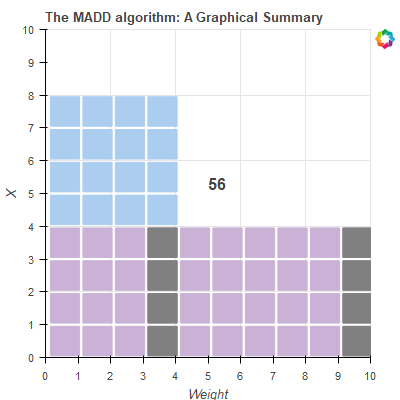
\includegraphics[width=200pt]{figures/rId37.png}}
	\caption{MADD: A description based on a geometric view of the MADD algorithm. Here we perform the operation $(4 \times 10)+(4 \times 4)$ right to left by accumulating the "height" at the index point}\label{fig:madd}
\end{figure}

The MADD algorithm originated from the use of discrete memory indexes as a simulation of time delays. As such the MADD algorithm is inspired by the temporal approach, but, its representation does not use time delays directly as the storage medium.

% \section{Temporal/Unary for Communication}\label{coms}
% 
% Interval codes have been exploited in the communication community in the form of DPIM \cite{Das1967PulseintervalM}, where the pulses delimit both the beginning and end of the encoded value. This method was heavily researched from the late sixties onwards \cite{marougi1983signal} \cite{kaluarachchi1997digital} \cite{sato1978pulse} and revisited by the optical community during the nineties \cite{ghassemlooy1998digital} \cite{ghassemlooy2000digital}. The scheme is very simple, and efficient in terms of the sparsity of the representation, with two spikes being able to represent any magnitude.
% 
% There are several further compelling advantages:
% 
% \begin{description}
% 
% 	\item [Bandwidth Efficiency] DPIM is more bandwidth-efficient than some other modulation schemes. This is because it doesn't require changes in amplitude or pulse width, which can demand more bandwidth.
% 	\item [Power Efficiency] Since DPIM doesn't rely on varying amplitude, it can be more power-efficient. Ghassemlooy states:
% 
% 	      \begin{quote}
% 		      For the same packet error performance, 4-bit DPIM has about a 5dB power advantage over OOK, but requires approximately 1dB more power than 4-bit PPM \cite{ghassemlooy2000digital}.
% 	      \end{quote}
% 
% 	      OOK is traditional bit encoding and PPM is Pulse Position Modulation (the same as DPIM but with a constant bit-width, hence pulses are not self-delimiting).
% 
% 	\item [Suitability for Optical Communication] DPIM is often used in optical communication systems because it can be implemented as light pulses.
% 	\item [Simplicity] The circuitry for DPIM can be simpler than other modulation schemes, as it only needs to control the timing of pulses.
% \end{description}
% 
% However, there has been a lack of adoption based on the following disadvantages:
% 
% \begin{description}
% 
% 	\item[Synchronization Complexity] One of the main challenges of DPIM is the requirement for precise synchronization between the transmitter and receiver. As with all temporal systems encoding and decoding require a very stable and accurate clock, which can add complexity and cost to the system.
% 	\item[Limited Data Rate] While DPIM can accommodate variable data rates, the practical data rate might be limited by the precision of the timing measurements.
% 	\item[Error Propagation] In some implementations of DPIM, errors in detecting one pulse interval can propagate and affect the detection of subsequent intervals.
% \end{description}
% 
% One point to note that affects how we might process temporal intervals in a computational setting is the use of ramp functions \cite{sato1978pulse}. A \textbf{ramp function}, also known as a saw-tooth wave or ramp waveform, is a type of signal where the voltage or current increases linearly with time, then abruptly drops back to its starting value, and repeats this cycle periodically. Figure \ref{fig:pim} gives a typical view of communication system using ramp functions to DPIM encoded data.
% 
% \begin{figure}[ht]
% 	\centerline{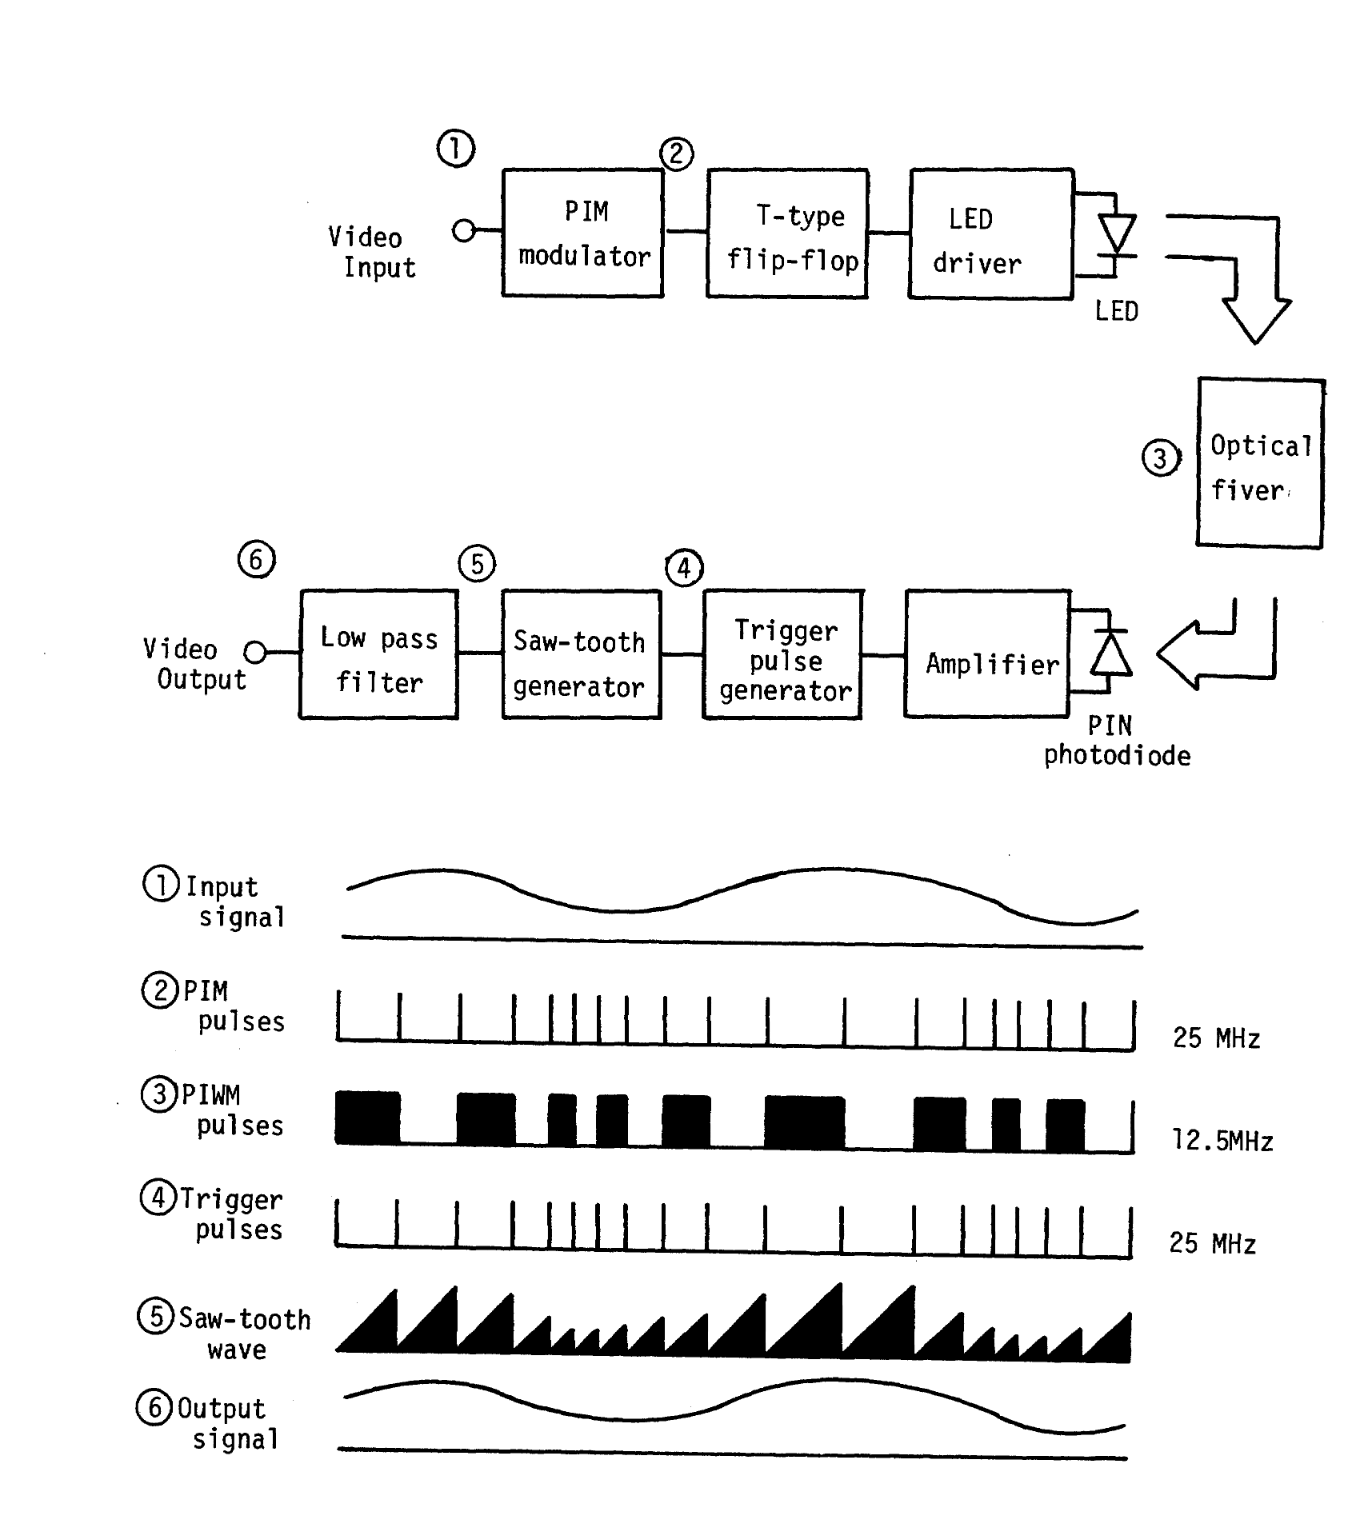
\includegraphics[width=300pt]{figures/PIM.png}}
% 	\caption{A communication system using ramps to encode and decode data. Taken from \cite{sato1978pulse}}\label{fig:pim}
% \end{figure}
% 
% DPIM has served as inspiration for many studies of neural information encoding in Neuroscience \cite{meister1999neural} \cite{rieke1995naturalistic} \cite{borst1999information}, Mackay's work \cite{MacKay1952} focused on the channel capacity of this simple model, and surprisingly they find that for a suitable set of constraints, time encoding outperforms single bit based information encoding.
% 

\section{Oscillatory Systems}\label{oscil}

An oscillatory computer utilises the dynamics of time-based coupled oscillators to perform computation.

Coupled Oscillators are a technique in non-linear dynamics that produce stable and predictable patterns of oscillation from the ensemble behaviours of many oscillators \cite{strogatz2001nonlinear}. The classic example of this is the firefly synchronisation problem \cite{buck1988synchronous} where fireflies in a forest synchronise their flashing patterns.

Unlike traditional computers, oscillatory computers encode and process information using the phase, frequency, or amplitude of oscillations. This approach is inspired by the observation that many biological systems, including the brain, use oscillatory dynamics for information processing and communication. For a review article and example see \cite{csaba2020coupled} and \cite{csaba2018perspectives}. Example systems include \cite{ring} \cite{delacour2021oscillatory} \cite{delacour2023mixed} \cite{corti2021networks} \cite{frady2019robust} \cite{maher2024highly}.

The advantages of oscillatory computers include:

\begin{itemize}
	\item Parallelism through the emerging dynamics of coupling.
	\item Energy Efficiency as they often rely on the natural dynamics of physical systems.
	\item Robustness to noise and variability, due to the collective dynamics of coupled oscillators.
\end{itemize}

\begin{figure}
	\centerline{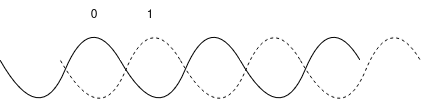
\includegraphics[width=200pt]{figures/oscil.png}}
	\caption{An example of how phase might encode a signal, in this case binary 0 and 1}\label{fig:fig2}
\end{figure}

Some of challenges associated with oscillatory computers include:

\begin{description}
	\item[Precision] The precision of computations in oscillatory computers may be limited by the inherent variability and noise in the oscillatory dynamics.
	\item[Programmability] Programming oscillatory computers can be difficult, as it requires the control of the complex dynamics of the coupling.
	\item[Scalability] Scaling up oscillatory computers to large numbers of oscillators can be difficult, as the dynamics can become increasingly complex and hard to control.
	\item[Interfacing] as with many systems discussed in this document interfacing with traditional digital systems is problematic, with similar problems to analog to digital conversion.
\end{description}

\section{Spiking Neural Networks and Neuromorphic Compute}\label{neuro}

Spiking Neural Networks (SNNs) \cite{maass2001pulsed} are a type of artificial neural network that more closely mimic the behavior of biological neural networks. SNNs are a key component of neuromorphic computing, which aims to develop hardware and software systems that mimic the structure and function of biological neural networks. This is extensive literature on neuromorphic hardware platforms, such as SpiNNaker \cite{furber2016large,furber2014spinnaker}, TrueNorth \cite{sawada2016truenorth}, Loihi \cite{davies2018loihi}, and BrainScale \cite{schmitt2017neuromorphic}. These platforms are optimized for low-power, real-time operation often outperforming their DL cousins in terms of energy usage \cite{reuther20}, but at the cost of conjoined hardware and software offerings.

Son's are explicitly temporal using spikes to define data, their key aspects are:

\begin{description}
	\item[Information Encoding] There are a variety of coding schemes, not just the ``width'' encoding discussed in this document. These are:
	      \begin{description}
		      \item[Rate Coding] Information is encoded in the average firing rate of neurons, similar to traditional ANNs.
		      \item[Temporal Coding] Information is encoded in the precise timing of individual spikes. This can include schemes like Time to First Spike (TTFS) or Rank Order Coding (ROC).
		      \item[Population Coding] Information is encoded in the collective activity of a group of neurons.
	      \end{description}
	      
	\item[Neuron Models] SNNs use more biologically plausible activation functions than ANNs. Some commonly used ones are:
	      \begin{description}
		      \item[Integrate-and-Fire (IF) Neurons] \cite{burkitt2006review} IF neurons integrate incoming spikes and fire an output spike when a threshold is reached. After firing, the neuron's membrane potential is reset.
		      \item[Leaky Integrate-and-Fire (LIF) Neurons] \cite{tal1997computing} LIF neurons are similar to IF neurons but include a leakage term that causes the membrane potential to decay over time.
		      \item[Hodgkin-Huxley Neurons] \cite{y2003computation} The Hodgkin-Huxley model is a detailed biophysical model that describes the dynamics of ion channels in the neuron membrane.
	      \end{description}
	\item[Synaptic Models] In SNNs, synapses can have dynamic behaviors, unlike the static weights used in traditional ANNs. This gives rise to a computationally richer and more compact pattern processing systems.
\end{description}

One of the most relevant applications of this idea is the work done by Hopfield \cite{hopfield1995pattern}. Hopfield's key insight was that the correct representation is the key to solving difficult problems:

\begin{quote}
	The choice of information representation is of vital importance in making a computation easy, as is illustrated by the question 'is 3630225 divisible by 7?'. If the number 3630225 is in base 10, answering this takes a bit of work. If the number 3630225 is in base 7, the answer is immediate from inspection of the last digit. The choice of representation for analogue information is equally important for neural computation. \cite{hopfield1995pattern}
\end{quote}

The main focus of this work is to mimic the behaviour of the olfactory system. This particular problem is termed the ``analog match'' problems, and whilst solvable via traditional logistic methods is more robust when recast as a coincidence problem. Figure \ref{fig:carlos} shows how the system functions, note that the data is log scaled.

\begin{figure}
	\centerline{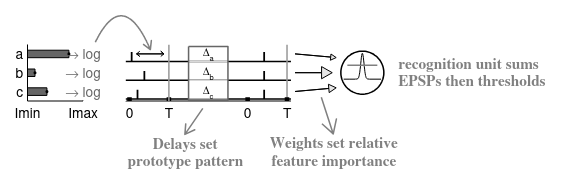
\includegraphics[width=300pt]{figures/carlos.png}}
	\caption{Computing with Action Potentials, taken from \cite{hopfield1995pattern}}\label{fig:carlos}
\end{figure}

% \section{Time Coding in the Human Brain} \label{app:brain}
% 
% The following section describes the major encoding methods utilised by the brain. This serves as background to the biological inspiration of the temporal coding strategy \cite{victor2000brain}.
% 
% \begin{figure}[ht]
% 	\centering
% 	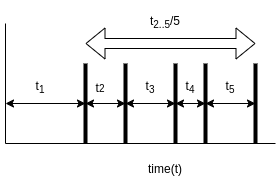
\includegraphics[width=200pt]{figures/rate.png}
% 	\caption{Rate and Time-to-first-spike Coding}
% 	\label{fig:rate}
% \end{figure}
% 
% Rate coding is the ``standard'' scheme for modelling neural signals computational \cite{rosenblatt1958perceptron}. The term is self-explanatory it is a count of the rate by which spikes arrive at a computational unit (see Figure \ref{fig:rate}). Averaging is robust and easy to model as a scalar value on traditional computers, however some questions exist as to whether a more immediate response is required from a (potentially threatening) stimulus, hence investigations into temporal and time to first spike encodings.
% 
% \subsection{Spike Timings}
% 
% In contrast to rate coding interval or spike coding utilises the exact time between two spikes as the magnitude of the signal. This model was first mentioned in the work of MacKay and McCullough \cite{MacKay1952} who focused on the channel rate of this simple model. Surprisingly, with neuron specific measurements, a maximum selective information capacity of about 2.9bit/msec is produced as opposed to 1bit/msec from a simple single-bit based encoding over a channel, where Information capacity ($C$ in bits/time) is given by:
% 
% $$C=\frac{2}{\Delta T(m+ r)} log_2(m- r)$$
% 
% where $\Delta T$ is the time resolution, $m=(T_m-T_r)/\Delta T$ approximately the range of data, and $r=\frac{T_r}{\Delta T}$ a lower bound.

\section{MeTTa: A Reflective Meta-Language for AGI}

MeTTa (Meta-Type Talk) \cite{goertzel2021metagraph} \cite{singularitynet2024mett} is the foundational programming language of OpenCog Hyperon \cite{opencogHyperon}, designed to support Artificial General Intelligence (AGI) through symbolic reasoning, introspection, and self-modifying code. It serves as a meta-language capable of defining and manipulating other languages and type systems.


\subsection{Core Features}

Reflective Metagraph Rewriting, Programs are represented as metagraphs---graphs of graphs---enabling recursive transformations and dynamic reasoning. MeTTa uses powerful pattern-matching and substitution primitives to infer and rewrite expressions. The language is syntactically sparse, allowing users to define custom logics and type systems. Grounding Support: Symbolic atoms can be linked to sensory or motor data, enabling embodied cognition.
 MeTTa programs can inspect and alter their own structure, supporting recursive self-improvement.

MeTTa operates as the lowest-level cognitive substrate in OpenCog Hyperon. It interfaces with the Distributed Atomspace (DAS), orchestrating reasoning, learning, and control. It replaces Atomese from OpenCog Classic with a more flexible and semantically rich alternative.

\section*{Applications}
\begin{itemize}
  \item Symbolic reasoning and logic programming
  \item Cognitive architecture modeling
  \item AGI-oriented introspection and learning
\end{itemize}

MeTTa, the meta-language of OpenCog Hyperon, supports probabilistic reasoning by enabling symbolic manipulation of uncertain knowledge through pattern rewriting and weighted truth values. Unlike traditional probabilistic programming languages that rely on explicit probability distributions, MeTTa operates over a hypergraph-based memory structure (the Distributed Atomspace), where each atom may carry a \textit{truth value}---a pair representing strength and confidence.

Probabilistic inference in MeTTa emerges from the interaction of three key mechanisms: (1) pattern matching over uncertain structures, (2) rule-based rewriting conditioned on probabilistic thresholds, and (3) recursive self-modification of inference strategies. These mechanisms allow MeTTa to encode Bayesian-like updates, fuzzy logic, and stochastic search within a unified symbolic substrate.

Rather than treating probability as a separate computational layer, MeTTa integrates it into the fabric of cognitive processes. For example, attention allocation, memory retrieval, and goal selection can all be guided by probabilistic heuristics encoded as MeTTa rules. This enables AGI systems to reason under uncertainty, adaptively revise beliefs, and simulate human-like cognition.

\section{Probabilistic Reasoning Example in MeTTa}
\section{Problem}
Decide whether to carry an umbrella based on the probability of rain. If the probability exceeds 0.6, the system recommends carrying an umbrella.

\section{MeTTa-Like Representation}

\begin{verbatim}
;; Define a probabilistic belief
(Probability (RainToday) 0.75)

;; Rule: If rain probability exceeds threshold, recommend umbrella
(If
  (GreaterThan (Probability (RainToday)) 0.6)
  (Then (Action CarryUmbrella))
)
\end{verbatim}

\section{Rewrite Logic}

\begin{verbatim}
;; Pattern to match
(Probability ?event ?p)
(GreaterThan ?p 0.6)

;; Rewrite result
(Action CarryUmbrella)
\end{verbatim}

\section{Truth Value Representation}

In OpenCog Hyperon, atoms may carry truth values as pairs of strength and confidence:

\begin{verbatim}
(RainToday)
:TruthValue (Strength 0.75) (Confidence 0.9)
\end{verbatim}

\section{Interpretation}
This structure allows MeTTa to reason symbolically over uncertain inputs and take action based on probabilistic thresholds. The system can generalize this logic to other decisions involving uncertainty.

\section{Critique}

The document provides an overview of four emerging areas in temporal computing: race logic, unary, oscillator, and neuromorphic. Each area presents unique challenges and opportunities for advancement in computational technology. To summarise the key points:

\begin{description}

	\item[Racelogic] is a practical and promising approach for utilising temporal data in computing. It's highlighted as one of the first methods to effectively a \textit{truly} temporal approach. Also, the work on temporal memories, significantly strengthens the case for this technology, and racelogic has already explored wide-ranging applications. Its scope in terms of arithmetic and compute based operations is currently limited to a few comparison operations, and hence there is a lack of insight into utilising race logic as a general-purpose computer.


	\item[Oscillatory Computing] Oscillator computing shows significant promise, with potential for high-speed operations in the range of 50-100 GHz. This technology could potentially offer a 10x improvement over current computing capabilities, however seems to be applicable to specialist problems rather than general compute.

	\item[Neuromorphic Computing] is the most mature technology among those reviewed. However, it is perhaps too literal in mimicking brain functionality, which may limit its potential. Our view is that time-based approaches should be emphasised over biological plausibility the analogy we draw is that of aircraft design, which draws inspiration from birds flight but in no way mimics the wing-flapping approach.


	\item[Unary Computing] Despite extensive past research, unary computing has been largely overlooked in recent years. It holds potential for reevaluation in light of advancements in AI and complex computing systems. The primary challenge lies in its memory footprint, as traditional memory doesn't scale well for unary representations. However, true temporal systems, ones which use time as data directly, are an avenue to alleviate this problem. Future research opportunities also include exploring unary signals with non-linear representations, which increase the efficiency of the subsequent computation. It is this methodology together with the discussion on pt-systems that provides the most synergy with the MeTTa language, and therefore the primary recommendation is to exploit this more fully.
\end{description}

We also briefly review Opencog and MeTTa with the overall conclusion being that a good area for synergy is the use of pt-systems as an underlying probabilistic framework for the MeTTa language. Thus, the pt-systems work is the most salient for further investigation, and where the scope should be more narrowly focused. Our hope is that a fully temporal stochastic system will allow us to position MeTTa as the  top level language for probabilistic stochastic computing. 
To finalise next steps, providing this report is accepted, investigations will start into how to implement a pt-system as low level hardware, using existing ideas discussed in this report, but alleviating the memory constraints by building a truly temporal system.  


\bibliographystyle{abbrv}
\bibliography{temporal}
\end{document}
